\documentclass[11pt, letterpaper]{article}

% Fonts and Encoding
\usepackage[utf8]{inputenc}
\usepackage[T1]{fontenc}
\usepackage{lmodern} % High-quality Latin Modern vector font

% Math and Symbols
\usepackage{amsmath, amssymb, amsthm, amsfonts, mathrsfs, mathtools}

% Layout and Geometry
\usepackage{geometry}
\geometry{letterpaper, margin=1in}
\setlength{\parindent}{0pt}
\setlength{\parskip}{0.6em}

% Formatting and Graphics
\usepackage{graphicx, xcolor, enumitem, booktabs, array, tabularx}

% TikZ for Illustrations
\usepackage{tikz}
\usetikzlibrary{arrows.meta, positioning, shapes.geometric, calc, backgrounds, matrix}

% Clickable Links and TOC
\usepackage{hyperref}
\hypersetup{
    colorlinks=true,
    linkcolor=blue,
    filecolor=magenta,      
    urlcolor=cyan,
    pdftitle={Advanced Mathematics Topic},
}

% Theorem Environments
\newtheorem{theorem}{Theorem}[section]
\newtheorem{lemma}[theorem]{Lemma}
\newtheorem{proposition}[theorem]{Proposition}
\newtheorem{corollary}[theorem]{Corollary}
\theoremstyle{definition}
\newtheorem{definition}{Definition}[section]
\newtheorem{axiom}{Axiom}[section]
\newtheorem{example}{Example}[section]
\theoremstyle{remark}
\newtheorem{remark}{Remark}[section]

% Custom Commands (Enforced standard notation)
\newcommand{\R}{\mathbb{R}}
\newcommand{\N}{\mathbb{N}}
\newcommand{\Z}{\mathbb{Z}}
\newcommand{\Q}{\mathbb{Q}}
\newcommand{\E}{\mathbb{E}}
\newcommand{\Prob}{\mathbb{P}}
\newcommand{\F}{\mathcal{F}}

\title{Solving Initial Value Problems with Laplace Transforms\\ \Large Comprehensive Problem Sets}
\author{Tashfeen Omran}
\date{November 5, 2026}

\begin{document}

\maketitle
\tableofcontents
\newpage

\section{Concept Checklist \& Question Mapping}

To ensure comprehensive mastery of solving Initial Value Problems (IVPs) using Laplace Transforms, the following concepts have been extracted from the source material and mapped to specific problems in this document.

\renewcommand{\arraystretch}{1.5}
\begin{tabularx}{\textwidth}{>{\raggedright\arraybackslash}X >{\centering\arraybackslash}p{3cm}}
\toprule
\textbf{Concept / Problem Type} & \textbf{Associated Questions} \\
\midrule
\textbf{1. Basic Constant Coefficient IVPs} (1st \& 2nd Order, PFD, Completing the Square) & 1, 2, 3, 4, 5, 6 \\
\addlinespace[4pt]
\textbf{2. Third-Order IVPs} (Higher-degree polynomials, repeated roots) & 7, 8, 9 \\
\addlinespace[4pt]
\textbf{3. Shifted Initial Conditions} (Transforming $t \to t+t_0$) & 10, 11, 12 \\
\addlinespace[4pt]
\textbf{4. Variable Coefficient ODEs} (Using $\mathcal{L}\{t y'\}$ and integrating factors) & 13, 14, 15, 16 \\
\addlinespace[4pt]
\textbf{5. Discontinuous Forcing Functions} (Heaviside step functions, Second Shifting Theorem) & 17, 18, 19, 20 \\
\addlinespace[4pt]
\textbf{6. Impulse Forcing} (Dirac Delta functions, instantaneous shocks) & 21, 22, 23 \\
\addlinespace[4pt]
\textbf{7. Systems of Linear ODEs} (Coupled equations, matrix-like elimination) & 24, 25, 26 \\
\addlinespace[4pt]
\textbf{8. General Solutions} (Symbolic initial conditions $a, b$) & 27, 28 \\
\addlinespace[4pt]
\textbf{9. Control Theory \& Real-World Modeling} (Transfer functions, impulse response) & 29 \\
\addlinespace[4pt]
\textbf{10. Diagnostic Testing} ("Find the Flaw" conceptual analysis) & 30 \\
\bottomrule
\end{tabularx}

\newpage

\section{Problem Sets}

\subsection{Basic Constant Coefficient IVPs}
\textbf{Problem 1.} Solve the initial value problem: $y'' - 3y' + 2y = 0; \quad y(0) = 1, \quad y'(0) = 1$.

\textbf{Problem 2.} Solve the initial value problem: $y'' + 4y = 3\sin(3t); \quad y(0) = 0, \quad y'(0) = 0$.

\textbf{Problem 3.} Solve the initial value problem: $y'' - 2y' + 5y = 0; \quad y(0) = 2, \quad y'(0) = 4$.

\textbf{Problem 4.} Solve the initial value problem: $y'' + 4y' + 4y = e^{-2t}; \quad y(0) = 1, \quad y'(0) = -1$.

\textbf{Problem 5.} Solve the initial value problem: $y'' - y' - 6y = 2e^{3t}; \quad y(0) = 0, \quad y'(0) = 0$.

\textbf{Problem 6.} Solve the initial value problem: $y'' + 2y' + 2y = e^{-t}\cos(t); \quad y(0) = 0, \quad y'(0) = 1$.

\subsection{Third-Order IVPs}
\textbf{Problem 7.} Solve the initial value problem: $y''' - y'' - 4y' + 4y = 0; \quad y(0) = 1, \quad y'(0) = 1, \quad y''(0) = -1$.

\textbf{Problem 8.} Solve the initial value problem: $y''' + y' = e^t; \quad y(0) = 0, \quad y'(0) = 0, \quad y''(0) = 1$.

\textbf{Problem 9.} Solve the initial value problem: $y''' - 3y'' + 3y' - y = 0; \quad y(0) = 1, \quad y'(0) = 0, \quad y''(0) = 0$.

\subsection{Shifted Initial Conditions}
\textbf{Problem 10.} Solve the initial value problem: $y'' - 4y = 0; \quad y(2) = 1, \quad y'(2) = 0$.

\textbf{Problem 11.} Solve the initial value problem: $y'' + y = t; \quad y(\pi) = 0, \quad y'(\pi) = 1$.

\textbf{Problem 12.} Solve the initial value problem: $y'' - 3y' + 2y = e^{t-1}; \quad y(1) = 0, \quad y'(1) = 1$.

\subsection{Variable Coefficient ODEs}
\textbf{Problem 13.} Solve the initial value problem: $ty'' + y' + ty = 0; \quad y(0) = 1, \quad y'(0) = 0$.

\textbf{Problem 14.} Solve the initial value problem: $ty'' + (1-t)y' + y = 0; \quad y(0) = 1, \quad y'(0) = -1$.

\textbf{Problem 15.} Solve the initial value problem: $y'' + 2ty' - 4y = 2; \quad y(0) = 0, \quad y'(0) = 0$.

\textbf{Problem 16.} Solve the initial value problem: $ty'' - ty' + y = 2; \quad y(0) = 2, \quad y'(0) = -1$.

\subsection{Discontinuous Forcing Functions}
\textbf{Problem 17.} Solve the initial value problem: $y'' + y = u(t-3); \quad y(0) = 0, \quad y'(0) = 0$.

\textbf{Problem 18.} Solve the initial value problem: $y'' - y = g(t); \quad y(0) = 1, \quad y'(0) = 0$, where $g(t) = t$ for $t < 1$, and $g(t) = 1$ for $t \ge 1$.

\textbf{Problem 19.} Solve the initial value problem: $y'' + 4y = \sin(t)u(t-\pi); \quad y(0) = 0, \quad y'(0) = 0$.

\textbf{Problem 20.} Solve the initial value problem: $y'' + 2y' + y = e^{-t}u(t-2); \quad y(0) = 0, \quad y'(0) = 0$.

\subsection{Impulse Forcing (Dirac Delta)}
\textbf{Problem 21.} Solve the initial value problem: $y'' + 9y = \delta(t-\pi/2); \quad y(0) = 0, \quad y'(0) = 0$.

\textbf{Problem 22.} Solve the initial value problem: $y'' - 2y' + 2y = e^t \delta(t-1); \quad y(0) = 0, \quad y'(0) = 0$.

\textbf{Problem 23.} Solve the initial value problem: $y'' + y = \delta(t-2\pi) + \delta(t-4\pi); \quad y(0) = 1, \quad y'(0) = 0$.

\subsection{Systems of Linear ODEs}
\textbf{Problem 24.} Solve the system: $x' = 3x - 4y$ and $y' = 4x + 3y$, with $x(0) = 1, \quad y(0) = 0$.

\textbf{Problem 25.} Solve the system: $x'' + y' = 0$ and $x' + y'' = 2$, with $x(0) = 0, \quad x'(0) = 0, \quad y(0) = 0, \quad y'(0) = 0$.

\textbf{Problem 26.} Solve the system: $x' = x + 2y$ and $y' = 2x + y + e^t$, with $x(0) = 0, \quad y(0) = 0$.

\subsection{General Solutions}
\textbf{Problem 27.} Solve the initial value problem: $y'' - 5y' + 6y = 0; \quad y(0) = a, \quad y'(0) = b$.

\textbf{Problem 28.} Solve the initial value problem: $y'' + \omega^2 y = 0; \quad y(0) = y_0, \quad y'(0) = v_0$.

\subsection{Control Theory \& Real-World Modeling}
\textbf{Problem 29.} A damped harmonic oscillator is governed by $Iy'' + \mu y' + ky = u(t)$. Find the impulse response $y(t)$ when the system is subjected to a unit impulse $u(t) = \delta(t)$, assuming $I=1, \mu=2, k=5$, and the system is initially at rest ($y(0)=0, y'(0)=0$).

\subsection{Diagnostic Testing: "Find the Flaw"}
\textbf{Problem 30.} Below is a flawed solution to an IVP. Identify the single critical conceptual or algebraic flaw, explain why it is wrong in one sentence, and provide the correct final answer.
\begin{quote}
\textbf{Problem:} Solve $y'' + 4y = u(t-\pi); \quad y(0) = 0, \quad y'(0) = 0$. \\
\textbf{Flawed Solution:}
\begin{align*}
\mathcal{L}\{y''\} + 4\mathcal{L}\{y\} &= \mathcal{L}\{u(t-\pi)\} \\
s^2 Y(s) + 4Y(s) &= \frac{e^{-\pi s}}{s} \\
Y(s) &= \frac{e^{-\pi s}}{s(s^2+4)} = e^{-\pi s} \left( \frac{1/4}{s} - \frac{s/4}{s^2+4} \right) \\
y(t) &= \frac{1}{4} u(t-\pi) - \frac{1}{4} \sin(2(t-\pi)) u(t-\pi)
\end{align*}
\end{quote}

\newpage

\section{Detailed Solutions}

\textbf{Solution 1.}
Apply the Laplace transform to both sides:
\[ [s^2 Y(s) - s(1) - 1] - 3[sY(s) - 1] + 2Y(s) = 0 \]
\[ (s^2 - 3s + 2)Y(s) - s - 1 + 3 = 0 \implies (s^2 - 3s + 2)Y(s) = s - 2 \]
\[ Y(s) = \frac{s - 2}{s^2 - 3s + 2} = \frac{s - 2}{(s - 1)(s - 2)} = \frac{1}{s - 1} \]
Applying the inverse Laplace transform:
\[ y(t) = e^t \]

\vspace{1em}
\textbf{Solution 2.}
Apply the Laplace transform:
\[ [s^2 Y(s) - 0 - 0] + 4Y(s) = \frac{9}{s^2 + 9} \]
\[ (s^2 + 4)Y(s) = \frac{9}{s^2 + 9} \implies Y(s) = \frac{9}{(s^2 + 4)(s^2 + 9)} \]
Use Partial Fraction Decomposition (PFD):
\[ \frac{9}{(s^2 + 4)(s^2 + 9)} = \frac{A}{s^2 + 4} + \frac{B}{s^2 + 9} \]
\[ A(s^2 + 9) + B(s^2 + 4) = 9 \]
Let $s^2 = -4 \implies A(5) = 9 \implies A = \frac{9}{5}$. Let $s^2 = -9 \implies B(-5) = 9 \implies B = -\frac{9}{5}$.
\[ Y(s) = \frac{9/5}{s^2 + 4} - \frac{9/5}{s^2 + 9} = \frac{9}{10} \left( \frac{2}{s^2 + 4} \right) - \frac{3}{5} \left( \frac{3}{s^2 + 9} \right) \]
\[ y(t) = \frac{9}{10}\sin(2t) - \frac{3}{5}\sin(3t) \]

\vspace{1em}
\textbf{Solution 3.}
Apply the Laplace transform:
\[ [s^2 Y(s) - 2s - 4] - 2[sY(s) - 2] + 5Y(s) = 0 \]
\[ (s^2 - 2s + 5)Y(s) - 2s = 0 \implies Y(s) = \frac{2s}{s^2 - 2s + 5} \]
Complete the square in the denominator: $s^2 - 2s + 5 = (s - 1)^2 + 4$.
\[ Y(s) = \frac{2s}{(s - 1)^2 + 4} = \frac{2(s - 1) + 2}{(s - 1)^2 + 4} = 2\frac{s - 1}{(s - 1)^2 + 2^2} + \frac{2}{(s - 1)^2 + 2^2} \]
\[ y(t) = 2e^t\cos(2t) + e^t\sin(2t) \]

\vspace{1em}
\textbf{Solution 4.}
Apply the Laplace transform:
\[ [s^2 Y(s) - s + 1] + 4[sY(s) - 1] + 4Y(s) = \frac{1}{s + 2} \]
\[ (s^2 + 4s + 4)Y(s) - s - 3 = \frac{1}{s + 2} \implies (s + 2)^2 Y(s) = \frac{1}{s + 2} + s + 3 \]
\[ Y(s) = \frac{1}{(s + 2)^3} + \frac{s + 3}{(s + 2)^2} = \frac{1}{(s + 2)^3} + \frac{(s + 2) + 1}{(s + 2)^2} = \frac{1}{(s + 2)^3} + \frac{1}{s + 2} + \frac{1}{(s + 2)^2} \]
Applying the inverse transform using $\mathcal{L}^{-1}\left\{\frac{n!}{s^{n+1}}\right\} = t^n$:
\[ y(t) = \frac{1}{2}t^2 e^{-2t} + e^{-2t} + t e^{-2t} \]

\vspace{1em}
\textbf{Solution 5.}
Apply the Laplace transform:
\[ [s^2 Y(s)] - [sY(s)] - 6Y(s) = \frac{2}{s - 3} \]
\[ (s^2 - s - 6)Y(s) = \frac{2}{s - 3} \implies (s - 3)(s + 2)Y(s) = \frac{2}{s - 3} \implies Y(s) = \frac{2}{(s - 3)^2(s + 2)} \]
PFD:
\[ \frac{2}{(s - 3)^2(s + 2)} = \frac{A}{s - 3} + \frac{B}{(s - 3)^2} + \frac{C}{s + 2} \]
Using Heaviside cover-up for $B$ and $C$:
$B = \frac{2}{3 + 2} = \frac{2}{5}$. $C = \frac{2}{(-2 - 3)^2} = \frac{2}{25}$.
To find $A$, let $s = 0$:
\[ \frac{2}{18} = \frac{A}{-3} + \frac{2/5}{9} + \frac{2/25}{2} \implies \frac{1}{9} = -\frac{A}{3} + \frac{2}{45} + \frac{1}{25} \implies A = -\frac{2}{25} \]
\[ Y(s) = -\frac{2/25}{s - 3} + \frac{2/5}{(s - 3)^2} + \frac{2/25}{s + 2} \]
\[ y(t) = -\frac{2}{25}e^{3t} + \frac{2}{5}te^{3t} + \frac{2}{25}e^{-2t} \]

\vspace{1em}
\textbf{Solution 6.}
Apply the Laplace transform:
\[ [s^2 Y(s) - 1] + 2[sY(s)] + 2Y(s) = \frac{s + 1}{(s + 1)^2 + 1} \]
\[ (s^2 + 2s + 2)Y(s) = 1 + \frac{s + 1}{(s + 1)^2 + 1} \implies ((s + 1)^2 + 1)Y(s) = 1 + \frac{s + 1}{(s + 1)^2 + 1} \]
\[ Y(s) = \frac{1}{(s + 1)^2 + 1} + \frac{s + 1}{((s + 1)^2 + 1)^2} \]
The first term is the transform of $e^{-t}\sin(t)$. The second term requires the property $\mathcal{L}\{t\sin(at)\} = \frac{2as}{(s^2+a^2)^2}$.
Here, $\mathcal{L}\{t\sin(t)\} = \frac{2s}{(s^2+1)^2}$. By the first shifting theorem, $\mathcal{L}\{e^{-t}t\sin(t)\} = \frac{2(s+1)}{((s+1)^2+1)^2}$.
Thus, the second term is $\frac{1}{2} \mathcal{L}\{t e^{-t}\sin(t)\}$.
\[ y(t) = e^{-t}\sin(t) + \frac{1}{2}t e^{-t}\sin(t) \]

\vspace{1em}
\textbf{Solution 7.}
Apply the Laplace transform:
\[ [s^3 Y - s^2(1) - s(1) - (-1)] - [s^2 Y - s(1) - 1] - 4[sY - 1] + 4Y = 0 \]
\[ (s^3 - s^2 - 4s + 4)Y - s^2 - s + 1 + s + 1 + 4 = 0 \]
\[ (s^2(s - 1) - 4(s - 1))Y - s^2 + 6 = 0 \implies (s - 1)(s - 2)(s + 2)Y = s^2 - 6 \]
\[ Y(s) = \frac{s^2 - 6}{(s - 1)(s - 2)(s + 2)} = \frac{A}{s - 1} + \frac{B}{s - 2} + \frac{C}{s + 2} \]
Cover-up method:
$A = \frac{1 - 6}{(1 - 2)(1 + 2)} = \frac{-5}{-3} = \frac{5}{3}$.
$B = \frac{4 - 6}{(2 - 1)(2 + 2)} = \frac{-2}{4} = -\frac{1}{2}$.
$C = \frac{4 - 6}{(-2 - 1)(-2 - 2)} = \frac{-2}{12} = -\frac{1}{6}$.
\[ y(t) = \frac{5}{3}e^t - \frac{1}{2}e^{2t} - \frac{1}{6}e^{-2t} \]

\vspace{1em}
\textbf{Solution 8.}
Apply the Laplace transform:
\[ [s^3 Y - 1] + [sY] = \frac{1}{s - 1} \implies (s^3 + s)Y = 1 + \frac{1}{s - 1} = \frac{s}{s - 1} \]
\[ s(s^2 + 1)Y = \frac{s}{s - 1} \implies Y(s) = \frac{1}{(s - 1)(s^2 + 1)} \]
PFD:
\[ \frac{1}{(s - 1)(s^2 + 1)} = \frac{A}{s - 1} + \frac{Bs + C}{s^2 + 1} \]
$A = \frac{1}{1^2 + 1} = \frac{1}{2}$.
$1 = \frac{1}{2}(s^2 + 1) + (Bs + C)(s - 1) \implies s^2\left(\frac{1}{2} + B\right) = 0 \implies B = -\frac{1}{2}$.
Constant term: $1 = \frac{1}{2} - C \implies C = -\frac{1}{2}$.
\[ Y(s) = \frac{1/2}{s - 1} - \frac{1}{2}\frac{s}{s^2 + 1} - \frac{1}{2}\frac{1}{s^2 + 1} \]
\[ y(t) = \frac{1}{2}e^t - \frac{1}{2}\cos(t) - \frac{1}{2}\sin(t) \]

\vspace{1em}
\textbf{Solution 9.}
Apply the Laplace transform:
\[ [s^3 Y - s^2] - 3[s^2 Y - s] + 3[sY - 1] - Y = 0 \]
\[ (s^3 - 3s^2 + 3s - 1)Y - s^2 + 3s - 3 = 0 \implies (s - 1)^3 Y = s^2 - 3s + 3 \]
\[ Y(s) = \frac{s^2 - 3s + 3}{(s - 1)^3} \]
Rewrite the numerator in terms of $(s - 1)$: $s^2 - 3s + 3 = (s - 1)^2 - s + 2 = (s - 1)^2 - (s - 1) + 1$.
\[ Y(s) = \frac{(s - 1)^2 - (s - 1) + 1}{(s - 1)^3} = \frac{1}{s - 1} - \frac{1}{(s - 1)^2} + \frac{1}{(s - 1)^3} \]
\[ y(t) = e^t - t e^t + \frac{1}{2}t^2 e^t \]

\vspace{1em}
\textbf{Solution 10.}
Shift the time variable. Let $w(t) = y(t + 2)$. Then $w(0) = y(2) = 1$ and $w'(0) = y'(2) = 0$.
The ODE becomes $w'' - 4w = 0$.
\[ s^2 W(s) - s - 4W(s) = 0 \implies (s^2 - 4)W(s) = s \implies W(s) = \frac{s}{s^2 - 4} \]
\[ w(t) = \cosh(2t) \]
Substitute back $y(t) = w(t - 2)$:
\[ y(t) = \cosh(2(t - 2)) \]

\vspace{1em}
\textbf{Solution 11.}
Let $w(t) = y(t + \pi)$. Then $w(0) = 0$ and $w'(0) = 1$.
The ODE becomes $w'' + w = (t + \pi)$.
\[ [s^2 W(s) - 1] + W(s) = \frac{1}{s^2} + \frac{\pi}{s} \implies (s^2 + 1)W(s) = 1 + \frac{1}{s^2} + \frac{\pi}{s} = \frac{s^2 + 1}{s^2} + \frac{\pi}{s} \]
\[ W(s) = \frac{1}{s^2} + \frac{\pi}{s(s^2 + 1)} = \frac{1}{s^2} + \pi\left(\frac{1}{s} - \frac{s}{s^2 + 1}\right) \]
\[ w(t) = t + \pi - \pi\cos(t) \]
Substitute back $y(t) = w(t - \pi)$:
\[ y(t) = (t - \pi) + \pi - \pi\cos(t - \pi) = t + \pi\cos(t) \]

\vspace{1em}
\textbf{Solution 12.}
Let $w(t) = y(t + 1)$. Then $w(0) = 0$ and $w'(0) = 1$.
The ODE becomes $w'' - 3w' + 2w = e^{(t+1)-1} = e^t$.
\[ [s^2 W(s) - 1] - 3[sW(s)] + 2W(s) = \frac{1}{s - 1} \]
\[ (s^2 - 3s + 2)W(s) = 1 + \frac{1}{s - 1} = \frac{s}{s - 1} \implies W(s) = \frac{s}{(s - 1)^2(s - 2)} \]
PFD: $\frac{s}{(s - 1)^2(s - 2)} = \frac{A}{s - 1} + \frac{B}{(s - 1)^2} + \frac{C}{s - 2}$.
$C = \frac{2}{(1)^2} = 2$. $B = \frac{1}{-1} = -1$.
Let $s = 0$: $0 = -A - 1 - 1 \implies A = -2$.
\[ W(s) = -\frac{2}{s - 1} - \frac{1}{(s - 1)^2} + \frac{2}{s - 2} \implies w(t) = -2e^t - t e^t + 2e^{2t} \]
Substitute back $y(t) = w(t - 1)$:
\[ y(t) = -2e^{t-1} - (t - 1)e^{t-1} + 2e^{2(t-1)} = -(t + 1)e^{t-1} + 2e^{2t-2} \]

\vspace{1em}
\textbf{Solution 13.}
Use the property $\mathcal{L}\{t f(t)\} = -F'(s)$.
\[ -\frac{d}{ds}[s^2 Y(s) - s(1) - 0] + [sY(s) - 1] - \frac{d}{ds}[Y(s)] = 0 \]
\[ -[2sY(s) + s^2 Y'(s) - 1] + sY(s) - 1 - Y'(s) = 0 \]
\[ -s^2 Y'(s) - 2sY(s) + 1 + sY(s) - 1 - Y'(s) = 0 \implies -(s^2 + 1)Y'(s) - sY(s) = 0 \]
\[ \frac{Y'(s)}{Y(s)} = -\frac{s}{s^2 + 1} \implies \ln Y(s) = -\frac{1}{2}\ln(s^2 + 1) + C \implies Y(s) = \frac{C}{\sqrt{s^2 + 1}} \]
By the Initial Value Theorem, $\lim_{s \to \infty} sY(s) = y(0) = 1$.
\[ \lim_{s \to \infty} \frac{Cs}{\sqrt{s^2 + 1}} = C = 1 \implies Y(s) = \frac{1}{\sqrt{s^2 + 1}} \]
This is the known transform of the Bessel function of the first kind of order zero:
\[ y(t) = J_0(t) \]

\vspace{1em}
\textbf{Solution 14.}
Apply the Laplace transform:
\[ -\frac{d}{ds}[s^2 Y - s] + [sY - 1] + \frac{d}{ds}[sY - 1] + Y = 0 \]
\[ -[2sY + s^2 Y' - 1] + sY - 1 + [Y + sY'] + Y = 0 \]
\[ Y'(-s^2 + s) + Y(-2s + s + 2) = 0 \implies Y'(s - s^2) + Y(2 - s) = 0 \]
\[ \frac{Y'}{Y} = \frac{s - 2}{s(1 - s)} = \frac{2 - s}{s(s - 1)} = -\frac{2}{s} + \frac{1}{s - 1} \]
Integrate both sides:
\[ \ln Y = -2\ln s + \ln(s - 1) + C \implies Y(s) = C\frac{s - 1}{s^2} \]
Using the Initial Value Theorem, $\lim_{s \to \infty} sY(s) = y(0) = 1 \implies C = 1$.
\[ Y(s) = \frac{s - 1}{s^2} = \frac{1}{s} - \frac{1}{s^2} \implies y(t) = 1 - t \]

\vspace{1em}
\textbf{Solution 15.}
Apply the Laplace transform:
\[ [s^2 Y] - 2\frac{d}{ds}[sY] - 4Y = \frac{2}{s} \implies s^2 Y - 2[Y + sY'] - 4Y = \frac{2}{s} \]
\[ -2sY' + (s^2 - 6)Y = \frac{2}{s} \implies Y' + \left(\frac{3}{s} - \frac{s}{2}\right)Y = -\frac{1}{s^2} \]
Find the integrating factor $\mu(s)$:
\[ \mu(s) = \exp\left(\int \left(\frac{3}{s} - \frac{s}{2}\right) ds\right) = \exp\left(3\ln s - \frac{s^2}{4}\right) = s^3 e^{-s^2/4} \]
Multiply the ODE by $\mu(s)$:
\[ (s^3 e^{-s^2/4} Y)' = -\frac{1}{s^2} \cdot s^3 e^{-s^2/4} = -s e^{-s^2/4} \]
Integrate both sides:
\[ s^3 e^{-s^2/4} Y = 2e^{-s^2/4} + C \implies Y(s) = \frac{2}{s^3} + \frac{C e^{s^2/4}}{s^3} \]
Since $\lim_{s \to \infty} Y(s) = 0$ for any valid transform, $C$ must be $0$ to prevent exponential growth.
\[ Y(s) = \frac{2}{s^3} \implies y(t) = t^2 \]

\vspace{1em}
\textbf{Solution 16.}
Apply the Laplace transform:
\[ -\frac{d}{ds}[s^2 Y - 2s + 1] + \frac{d}{ds}[sY - 2] + Y = \frac{2}{s} \]
\[ -[2sY + s^2 Y' - 2] + [Y + sY'] + Y = \frac{2}{s} \]
\[ Y'(s - s^2) + Y(2 - 2s) + 2 = \frac{2}{s} \implies s(1 - s)Y' + 2(1 - s)Y = \frac{2}{s} - 2 = \frac{2(1 - s)}{s} \]
Divide by $(1 - s)$ (assuming $s \neq 1$):
\[ sY' + 2Y = \frac{2}{s} \implies Y' + \frac{2}{s}Y = \frac{2}{s^2} \]
Integrating factor $\mu(s) = s^2$:
\[ (s^2 Y)' = 2 \implies s^2 Y = 2s + C \implies Y(s) = \frac{2}{s} + \frac{C}{s^2} \]
Inverse transform: $y(t) = 2 + Ct$. Since $y'(0) = -1$, we have $C = -1$.
\[ y(t) = 2 - t \]

\vspace{1em}
\textbf{Solution 17.}
Apply the Laplace transform:
\[ (s^2 + 1)Y(s) = \frac{e^{-3s}}{s} \implies Y(s) = e^{-3s}\frac{1}{s(s^2 + 1)} \]
PFD on the rational part: $\frac{1}{s(s^2 + 1)} = \frac{1}{s} - \frac{s}{s^2 + 1}$.
The inverse transform of this part is $1 - \cos(t)$.
Using the Second Shifting Theorem $\mathcal{L}^{-1}\{e^{-as}F(s)\} = f(t - a)u(t - a)$:
\[ y(t) = (1 - \cos(t - 3))u(t - 3) \]

\vspace{1em}
\textbf{Solution 18.}
First, rewrite $g(t)$ using Heaviside step functions:
\[ g(t) = t + (1 - t)u(t - 1) \]
Apply the Laplace transform to $g(t)$:
\[ \mathcal{L}\{g(t)\} = \frac{1}{s^2} + e^{-s}\mathcal{L}\{1 - (t + 1)\} = \frac{1}{s^2} - \frac{e^{-s}}{s^2} \]
Now transform the ODE:
\[ [s^2 Y(s) - s] - Y(s) = \frac{1}{s^2} - \frac{e^{-s}}{s^2} \implies (s^2 - 1)Y(s) = s + \frac{1}{s^2} - \frac{e^{-s}}{s^2} \]
\[ Y(s) = \frac{s}{s^2 - 1} + \frac{1}{s^2(s^2 - 1)} - e^{-s}\frac{1}{s^2(s^2 - 1)} \]
PFD for $\frac{1}{s^2(s^2 - 1)} = \frac{1}{s^2 - 1} - \frac{1}{s^2}$.
\[ Y(s) = \frac{s}{s^2 - 1} + \frac{1}{s^2 - 1} - \frac{1}{s^2} - e^{-s}\left(\frac{1}{s^2 - 1} - \frac{1}{s^2}\right) \]
Inverse transform:
\[ y(t) = \cosh(t) + \sinh(t) - t - (\sinh(t - 1) - (t - 1))u(t - 1) \]
\[ y(t) = e^t - t - (\sinh(t - 1) - t + 1)u(t - 1) \]

\begin{center}
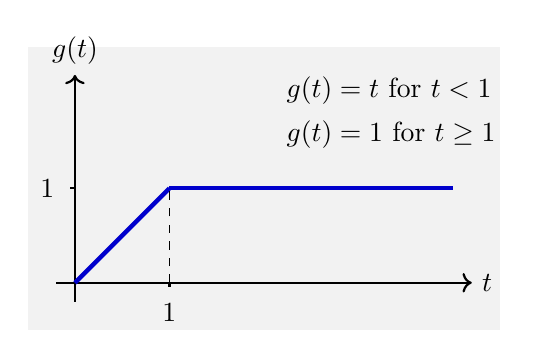
\begin{tikzpicture}[scale=1.2]
    \draw[fill=gray!10, draw=none] (-0.5, -0.5) rectangle (4.5, 2.5);
    \draw[thick, ->] (-0.2, 0) -- (4.2, 0) node[right] {$t$};
    \draw[thick, ->] (0, -0.2) -- (0, 2.2) node[above] {$g(t)$};
    
    \draw[ultra thick, blue!80!black] (0,0) -- (1,1);
    \draw[ultra thick, blue!80!black] (1,1) -- (4,1);
    
    \draw[dashed] (1,0) -- (1,1);
    \draw[thick] (1,0) -- (1,-0.05) node[below=2pt] {$1$};
    \draw[thick] (0,1) -- (-0.05,1) node[left=2pt] {$1$};
    
    \node[align=left, inner sep=8pt, anchor=west] at (2, 1.8) {
        $g(t) = t$ for $t < 1$ \\[4pt]
        $g(t) = 1$ for $t \ge 1$
    };
\end{tikzpicture}
\end{center}

\vspace{1em}
\textbf{Solution 19.}
Transform the RHS using the Second Shifting Theorem:
\[ \mathcal{L}\{\sin(t)u(t - \pi)\} = e^{-\pi s}\mathcal{L}\{\sin(t + \pi)\} = e^{-\pi s}\mathcal{L}\{-\sin(t)\} = -\frac{e^{-\pi s}}{s^2 + 1} \]
Transform the ODE:
\[ (s^2 + 4)Y(s) = -\frac{e^{-\pi s}}{s^2 + 1} \implies Y(s) = -e^{-\pi s}\frac{1}{(s^2 + 1)(s^2 + 4)} \]
PFD: $\frac{1}{(s^2 + 1)(s^2 + 4)} = \frac{1/3}{s^2 + 1} - \frac{1/3}{s^2 + 4}$.
\[ Y(s) = e^{-\pi s}\left(\frac{1/3}{s^2 + 4} - \frac{1/3}{s^2 + 1}\right) \]
Inverse transform:
\[ y(t) = \left[ \frac{1}{6}\sin(2(t - \pi)) - \frac{1}{3}\sin(t - \pi) \right] u(t - \pi) \]
Since $\sin(2(t - \pi)) = \sin(2t)$ and $\sin(t - \pi) = -\sin(t)$:
\[ y(t) = \left[ \frac{1}{6}\sin(2t) + \frac{1}{3}\sin(t) \right] u(t - \pi) \]

\vspace{1em}
\textbf{Solution 20.}
Transform the RHS:
\[ \mathcal{L}\{e^{-t}u(t - 2)\} = e^{-2s}\mathcal{L}\{e^{-(t + 2)}\} = e^{-2s}e^{-2}\frac{1}{s + 1} \]
Transform the ODE:
\[ (s^2 + 2s + 1)Y(s) = e^{-2(s + 1)}\frac{1}{s + 1} \implies (s + 1)^2 Y(s) = e^{-2(s + 1)}\frac{1}{s + 1} \]
\[ Y(s) = e^{-2s}e^{-2}\frac{1}{(s + 1)^3} \]
The inverse transform of $\frac{1}{(s + 1)^3}$ is $\frac{1}{2}t^2 e^{-t}$.
Applying the shift:
\[ y(t) = e^{-2} \left[ \frac{1}{2}(t - 2)^2 e^{-(t - 2)} \right] u(t - 2) = \frac{1}{2}(t - 2)^2 e^{-t} u(t - 2) \]

\vspace{1em}
\textbf{Solution 21.}
Apply the Laplace transform:
\[ (s^2 + 9)Y(s) = e^{-\pi s / 2} \implies Y(s) = e^{-\pi s / 2}\frac{1}{s^2 + 9} \]
Inverse transform:
\[ y(t) = \frac{1}{3}\sin\left(3\left(t - \frac{\pi}{2}\right)\right)u\left(t - \frac{\pi}{2}\right) = \frac{1}{3}\cos(3t)u\left(t - \frac{\pi}{2}\right) \]

\begin{center}
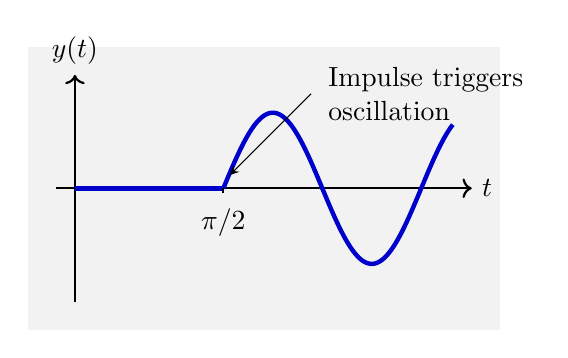
\begin{tikzpicture}[scale=1.2]
    \draw[fill=gray!10, draw=none] (-0.5, -1.5) rectangle (4.5, 1.5);
    \draw[thick, ->] (-0.2, 0) -- (4.2, 0) node[right] {$t$};
    \draw[thick, ->] (0, -1.2) -- (0, 1.2) node[above] {$y(t)$};
    
    \draw[ultra thick, blue!80!black, domain=1.57:4, samples=100] plot (\x, {0.8*cos(3*\x r)});
    \draw[ultra thick, blue!80!black] (0,0) -- (1.57,0);
    
    \draw[thick] (1.57,0) -- (1.57,-0.05) node[below=2pt] {$\pi/2$};
    \draw[->, >=stealth, shorten >=2pt] (2.5, 1) -- (1.6, 0.1);
    \node[align=left, inner sep=6pt, anchor=west] at (2.5, 1) {Impulse triggers \\ oscillation};
\end{tikzpicture}
\end{center}

\vspace{1em}
\textbf{Solution 22.}
Simplify the RHS using the sifting property of the Dirac delta: $e^t \delta(t - 1) = e^1 \delta(t - 1) = e\delta(t - 1)$.
Apply the Laplace transform:
\[ (s^2 - 2s + 2)Y(s) = e \cdot e^{-s} \implies Y(s) = e^{1 - s}\frac{1}{(s - 1)^2 + 1} \]
Inverse transform:
\[ y(t) = e \cdot e^{(t - 1)}\sin(t - 1)u(t - 1) = e^t \sin(t - 1)u(t - 1) \]

\vspace{1em}
\textbf{Solution 23.}
Apply the Laplace transform:
\[ [s^2 Y(s) - s] + Y(s) = e^{-2\pi s} + e^{-4\pi s} \implies (s^2 + 1)Y(s) = s + e^{-2\pi s} + e^{-4\pi s} \]
\[ Y(s) = \frac{s}{s^2 + 1} + \frac{e^{-2\pi s}}{s^2 + 1} + \frac{e^{-4\pi s}}{s^2 + 1} \]
Inverse transform:
\[ y(t) = \cos(t) + \sin(t - 2\pi)u(t - 2\pi) + \sin(t - 4\pi)u(t - 4\pi) \]
Since $\sin(t - 2\pi) = \sin(t)$ and $\sin(t - 4\pi) = \sin(t)$:
\[ y(t) = \cos(t) + \sin(t)u(t - 2\pi) + \sin(t)u(t - 4\pi) \]

\vspace{1em}
\textbf{Solution 24.}
Apply the Laplace transform to both equations:
\[ sX(s) - 1 = 3X(s) - 4Y(s) \implies (s - 3)X(s) + 4Y(s) = 1 \]
\[ sY(s) = 4X(s) + 3Y(s) \implies -4X(s) + (s - 3)Y(s) = 0 \implies X(s) = \frac{s - 3}{4}Y(s) \]
Substitute $X(s)$ into the first equation:
\[ (s - 3)\left(\frac{s - 3}{4}Y(s)\right) + 4Y(s) = 1 \implies \left((s - 3)^2 + 16\right)Y(s) = 4 \]
\[ Y(s) = \frac{4}{(s - 3)^2 + 16} \implies y(t) = e^{3t}\sin(4t) \]
Now find $X(s)$:
\[ X(s) = \frac{s - 3}{4} \left( \frac{4}{(s - 3)^2 + 16} \right) = \frac{s - 3}{(s - 3)^2 + 16} \implies x(t) = e^{3t}\cos(4t) \]

\vspace{1em}
\textbf{Solution 25.}
Apply the Laplace transform:
\[ s^2 X(s) + sY(s) = 0 \implies sX(s) + Y(s) = 0 \implies Y(s) = -sX(s) \]
\[ sX(s) + s^2 Y(s) = \frac{2}{s} \]
Substitute $Y(s)$:
\[ sX(s) + s^2(-sX(s)) = \frac{2}{s} \implies X(s)(s - s^3) = \frac{2}{s} \implies X(s) = \frac{2}{s^2(1 - s^2)} \]
PFD for $X(s)$:
\[ \frac{2}{s^2(1 - s)(1 + s)} = \frac{2}{s^2} + \frac{2}{1 - s^2} = \frac{2}{s^2} + \frac{1}{1 - s} + \frac{1}{1 + s} = \frac{2}{s^2} - \frac{1}{s - 1} + \frac{1}{s + 1} \]
\[ x(t) = 2t - e^t + e^{-t} = 2t - 2\sinh(t) \]
Now for $Y(s)$:
\[ Y(s) = -sX(s) = -\frac{2}{s(1 - s^2)} = -\frac{2}{s} + \frac{1}{1 - s} - \frac{1}{1 + s} = -\frac{2}{s} - \frac{1}{s - 1} - \frac{1}{s + 1} \]
\[ y(t) = -2 - e^t - e^{-t} = -2 - 2\cosh(t) \]

\vspace{1em}
\textbf{Solution 26.}
Apply the Laplace transform:
\[ sX(s) = X(s) + 2Y(s) \implies (s - 1)X(s) = 2Y(s) \implies X(s) = \frac{2}{s - 1}Y(s) \]
\[ sY(s) = 2X(s) + Y(s) + \frac{1}{s - 1} \implies -2X(s) + (s - 1)Y(s) = \frac{1}{s - 1} \]
Substitute $X(s)$:
\[ -2\left(\frac{2}{s - 1}Y(s)\right) + (s - 1)Y(s) = \frac{1}{s - 1} \implies \frac{-4 + (s - 1)^2}{s - 1}Y(s) = \frac{1}{s - 1} \]
\[ ((s - 1)^2 - 4)Y(s) = 1 \implies Y(s) = \frac{1}{s^2 - 2s - 3} = \frac{1}{(s - 3)(s + 1)} \]
PFD for $Y(s)$:
\[ Y(s) = \frac{1/4}{s - 3} - \frac{1/4}{s + 1} \implies y(t) = \frac{1}{4}e^{3t} - \frac{1}{4}e^{-t} \]
Now for $X(s)$:
\[ X(s) = \frac{2}{s - 1} \frac{1}{(s - 3)(s + 1)} = \frac{A}{s - 1} + \frac{B}{s - 3} + \frac{C}{s + 1} \]
$A = \frac{2}{(-2)(2)} = -\frac{1}{2}$. $B = \frac{2}{(2)(4)} = \frac{1}{4}$. $C = \frac{2}{(-2)(-4)} = \frac{1}{4}$.
\[ x(t) = -\frac{1}{2}e^t + \frac{1}{4}e^{3t} + \frac{1}{4}e^{-t} \]

\vspace{1em}
\textbf{Solution 27.}
Apply the Laplace transform:
\[ [s^2 Y(s) - as - b] - 5[sY(s) - a] + 6Y(s) = 0 \]
\[ (s^2 - 5s + 6)Y(s) = as + b - 5a \implies Y(s) = \frac{as + b - 5a}{(s - 2)(s - 3)} \]
PFD:
\[ \frac{as + b - 5a}{(s - 2)(s - 3)} = \frac{A}{s - 2} + \frac{B}{s - 3} \]
$A = \frac{2a + b - 5a}{-1} = 3a - b$.
$B = \frac{3a + b - 5a}{1} = b - 2a$.
\[ y(t) = (3a - b)e^{2t} + (b - 2a)e^{3t} \]

\vspace{1em}
\textbf{Solution 28.}
Apply the Laplace transform:
\[ [s^2 Y(s) - y_0 s - v_0] + \omega^2 Y(s) = 0 \implies (s^2 + \omega^2)Y(s) = y_0 s + v_0 \]
\[ Y(s) = y_0 \frac{s}{s^2 + \omega^2} + \frac{v_0}{\omega} \frac{\omega}{s^2 + \omega^2} \]
\[ y(t) = y_0 \cos(\omega t) + \frac{v_0}{\omega} \sin(\omega t) \]

\vspace{1em}
\textbf{Solution 29.}
Substitute the given constants: $y'' + 2y' + 5y = \delta(t)$.
Apply the Laplace transform:
\[ (s^2 + 2s + 5)Y(s) = 1 \implies Y(s) = \frac{1}{s^2 + 2s + 5} = \frac{1}{(s + 1)^2 + 4} \]
Inverse transform:
\[ y(t) = \frac{1}{2}e^{-t}\sin(2t) \]

\begin{center}
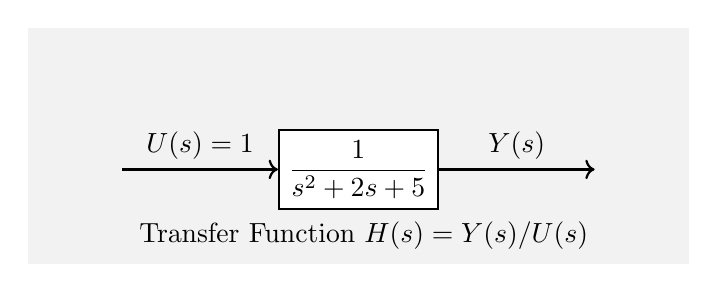
\begin{tikzpicture}[scale=1.2]
    \draw[fill=gray!10, draw=none] (-1, -1) rectangle (6, 1.5);
    
    \node[draw, thick, fill=white, minimum width=2cm, minimum height=1cm] (plant) at (2.5, 0) {$\displaystyle \frac{1}{s^2 + 2s + 5}$};
    
    \draw[->, thick] (0, 0) -- (plant.west) node[midway, above] {$U(s) = 1$};
    \draw[->, thick] (plant.east) -- (5, 0) node[midway, above] {$Y(s)$};
    
    \node[align=left, inner sep=6pt, anchor=west] at (0, -0.7) {Transfer Function $H(s) = Y(s)/U(s)$};
\end{tikzpicture}
\end{center}

\vspace{1em}
\textbf{Solution 30.}
\textbf{Flaw Identification:} The inverse Laplace transform of $\frac{s}{s^2+4}$ is $\cos(2t)$, not $\sin(2t)$.
\textbf{Correct Final Answer:}
\[ Y(s) = e^{-\pi s} \left( \frac{1/4}{s} - \frac{1}{4}\frac{s}{s^2+4} \right) \]
\[ y(t) = \frac{1}{4} u(t-\pi) - \frac{1}{4} \cos(2(t-\pi)) u(t-\pi) \]
Since $\cos(2(t-\pi)) = \cos(2t - 2\pi) = \cos(2t)$, this simplifies to:
\[ y(t) = \frac{1}{4}(1 - \cos(2t))u(t-\pi) \]

\newpage

\section{Concept Checklist \& Question Mapping (Review)}

\renewcommand{\arraystretch}{1.5}
\begin{tabularx}{\textwidth}{>{\raggedright\arraybackslash}X >{\centering\arraybackslash}p{3cm}}
\toprule
\textbf{Concept / Problem Type} & \textbf{Associated Questions} \\
\midrule
\textbf{1. Basic Constant Coefficient IVPs} (1st \& 2nd Order, PFD, Completing the Square) & 1, 2, 3, 4, 5, 6 \\
\addlinespace[4pt]
\textbf{2. Third-Order IVPs} (Higher-degree polynomials, repeated roots) & 7, 8, 9 \\
\addlinespace[4pt]
\textbf{3. Shifted Initial Conditions} (Transforming $t \to t+t_0$) & 10, 11, 12 \\
\addlinespace[4pt]
\textbf{4. Variable Coefficient ODEs} (Using $\mathcal{L}\{t y'\}$ and integrating factors) & 13, 14, 15, 16 \\
\addlinespace[4pt]
\textbf{5. Discontinuous Forcing Functions} (Heaviside step functions, Second Shifting Theorem) & 17, 18, 19, 20 \\
\addlinespace[4pt]
\textbf{6. Impulse Forcing} (Dirac Delta functions, instantaneous shocks) & 21, 22, 23 \\
\addlinespace[4pt]
\textbf{7. Systems of Linear ODEs} (Coupled equations, matrix-like elimination) & 24, 25, 26 \\
\addlinespace[4pt]
\textbf{8. General Solutions} (Symbolic initial conditions $a, b$) & 27, 28 \\
\addlinespace[4pt]
\textbf{9. Control Theory \& Real-World Modeling} (Transfer functions, impulse response) & 29 \\
\addlinespace[4pt]
\textbf{10. Diagnostic Testing} ("Find the Flaw" conceptual analysis) & 30 \\
\bottomrule
\end{tabularx}

\end{document}